\documentclass[dvipdfmx]{jsarticle}
\usepackage{url}
\usepackage{listings}
\usepackage[dvipdfmx]{graphicx}
\usepackage{here}
\usepackage{ascmac}\usepackage{listings, jlisting, color}
\definecolor{OliveGreen}{rgb}{0.0,0.6,0.0}
\definecolor{Orenge}{rgb}{0.89,0.55,0}
\definecolor{SkyBlue}{rgb}{0.28, 0.28, 0.95}
\lstset{
  language={C++}, % 言語の指定
  basicstyle={\ttfamily},
  identifierstyle={\small},
  commentstyle={\smallitshape},
  keywordstyle={\small\bfseries},
  ndkeywordstyle={\small},
  stringstyle={\small\ttfamily},
  frame={tb},
  breaklines=true,
  columns=[l]{fullflexible},
  numbers=left,
  xrightmargin=0zw,
  xleftmargin=3zw,
  numberstyle={\scriptsize},
  stepnumber=1,
  numbersep=1zw,
  lineskip=-0.5ex,
  keywordstyle={\color{SkyBlue}},     %キーワード(int, ifなど)の書体指定
  commentstyle={\color{OliveGreen}},  %注釈の書体
  stringstyle=\color{Orenge}          %文字列
}

\begin{document}
\title{課題9}
\author{ロボ団マスターコース}
\maketitle

\section{はじめに}
前回から授業で取り組んでいるPython3問題.
今回の授業でも行うよ!\\
アルゴリズムの能力とPythonのプログラミング力が養われるから頑張ろう!\\
Pythonを動かすことができるサイト:\url{https://www.tutorialspoint.com/execute_python_online.php}
\section{問題}
\subsection{}
すぬけ君は 1,2,3の番号がついた3つのマスからなるマス目を持っています.
すぬけ君は 1 が書かれたマスにビー玉を置きます.ビー玉が置かれるマスがいくつあるか求めよう!
\begin{figure}[H]
  \centering
  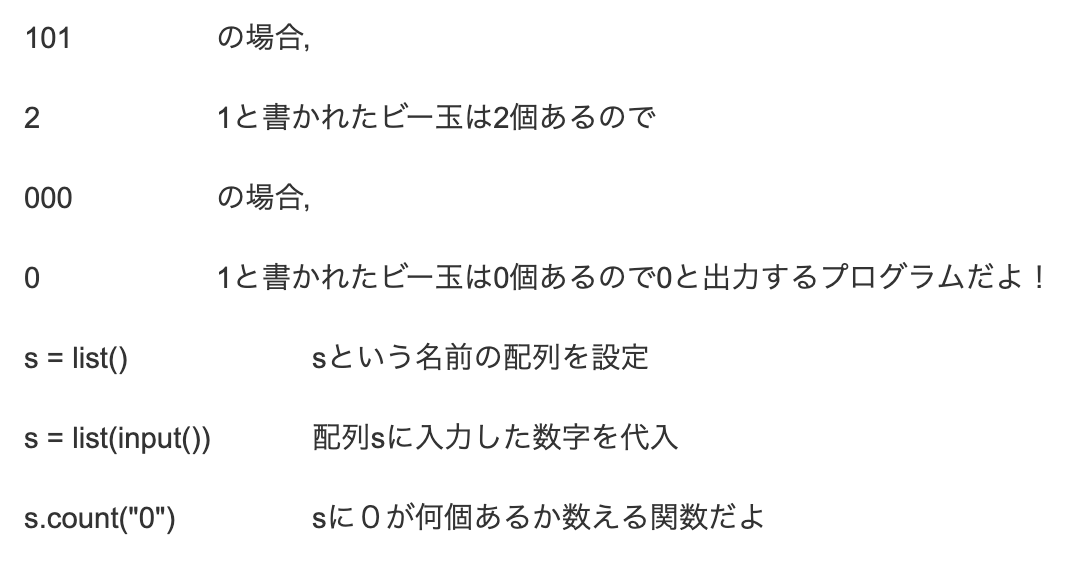
\includegraphics[width=15cm]{9.png}
\end{figure}
\subsection{}
すぬけ君は,黒板に書かれている整数がすべて偶数であるとき,書かれている整数すべてを2で割ったものに置き換える事ができます.すぬけ君は最大で何回操作を行うことができるかを求めよう!
\begin{figure}[H]
  \centering
  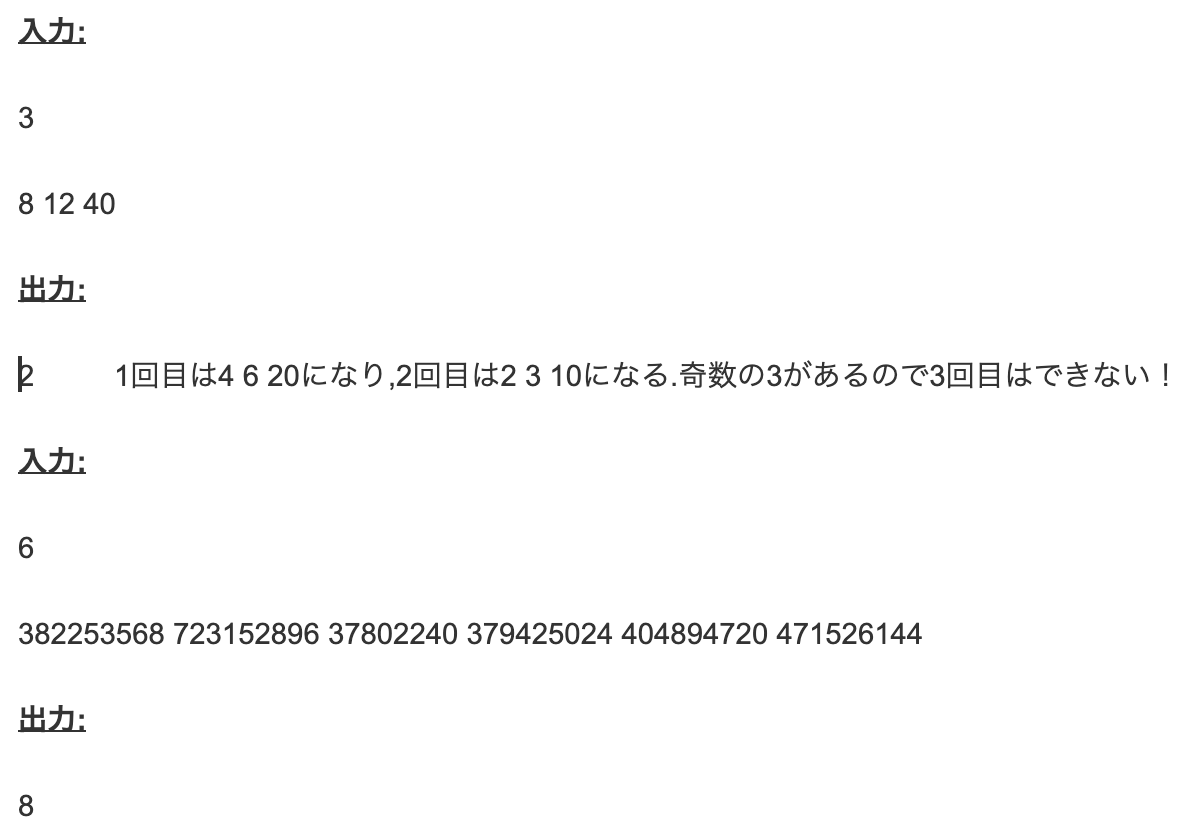
\includegraphics[width=15cm]{9-1.png}
\end{figure}
\subsection{}
もつお君は,500円玉をA枚,100円玉をB枚,50円玉をC枚持っています.これらの硬貨の中から何枚かを選び,合計金額をちょうどX円にする方法は何通りありますか.同じ種類の硬貨どうしは区別できません.2 通りの硬貨の選び方は,ある種類の硬貨についてその硬貨を選ぶ枚数が異なるとき区別されます.
\begin{figure}[H]
  \centering
  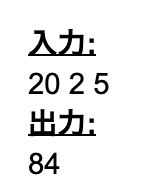
\includegraphics[width=2cm]{9-3.png}
\end{figure}
\subsection{}
1以上N以下の整数のうち,10進法での各桁の和がA以上B以下であるものの総和を求めよう!

20以下の整数のうち,各桁の和が2以上5以下なのは2,3,4,5,11,12,13,14,20.これらの合計は84なので84を出力しよう.
\subsection{}
古くからある日本の文化として海外でも有名な俳句というものがあります.
俳句は5,7,5で表現されることから五七五とも呼ばれます.\\
そんな俳句が大好きなもつお君がいました.
しかし,もつお君はまだ俳句を初めてまもないのでよく文字数を間違えてしまいます.\\
3つの文節の並びの文字数がそれぞれ 5,7,5となるようにこの順番で並んでいるときには俳句といえます.
5,5,7でも並び変えれば俳句になるので俳句です.\\
これらを判定するプログラムを作ってみましょう!\\\\
俳句の場合は”HAIKU!”と表示し,俳句ではない場合は”MOTSUO!”と表示しよう!\\
575の場合"HAIKU!"となります\\
557の場合”HAIKU!”となります\\
577の場合”MOTSUO!”となります\\
前回ならったinput()関数や
\begin{lstlisting} 
s=input()
print("{}".format(s))
\end{lstlisting}
if文をつかって解いて見よう!!
\begin{lstlisting} 
if n==1:
	print("1です")
else:
	print("1ではないです")
\end{lstlisting}

\subsection{}
ロボ団春日井校の生徒さんへ宿題を出すことにしました.
N人の生徒さんを1列に並んでもらい,1人目には1つ宿題を出し,2人目には2つ宿題を出します.\\
この要領でN人目にはN個の宿題を出すことにします.
すぬけ君の順番を入力していくつ宿題を出すか表示するプログラムを作ろう!\\
\subsection{}
1軒のホテルがあります。 このホテルの宿泊費は、次のようになっています。
最初のK泊までは,1
 泊あたり 
X
 円
K
+
1
 泊目以降は、
1
 泊あたり 
Y
 円
高橋君は、このホテルに 
N
 泊連続で宿泊することにしました。 高橋君の宿泊費は合計で何円になるか求めてください。


\end{document}
